\begin{frame}
	\myheading{Module 9.1 : A quick recap of training deep neural networks}
\end{frame}

%%%%%%%%%%%%%%%%%%%%%%%%%%%%%%%%%%%%%%%%%%%%%%%%%%%%%%%%%%%%%%%%%%%%%%%%%%%%%%

\begin{frame}
	
	\begin{columns}
		\column{0.35\textwidth}
		\begin{overlayarea}{\textwidth}{\textheight}
			
			\begin{center}
				
				\only<1-10>
				{
					\tikzstyle{input_neuron}=[circle,draw=red!50,fill=orange!10,thick,minimum size=.2mm]
\tikzstyle{hidden_neuron}=[circle,draw=blue!50,fill=blue!10,thick,minimum size=1mm]
\tikzstyle{output_neuron}=[circle,draw=green!50,fill=green!20,thick,minimum size=1mm]
\tikzstyle{input}=[circle,draw=black!50,fill=black!20,thick,minimum size=.2mm]

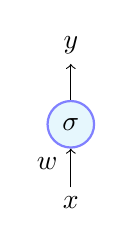
\begin{tikzpicture}

	\node (input0) at (10,5)  {$x$};
	\node [hidden_neuron] (neuron1) at (10,6)  {$\sigma$};
	\node (formula) at (9.7,5.5) {$w$};
	\node (output0)  at (10,7) {$y$};	
	\draw [->] (input0) -- (neuron1);
	\draw [->] (neuron1) -- (output0);
	
\end{tikzpicture}
				}
				
				\only<6-10>{
					\vspace{.65in}
					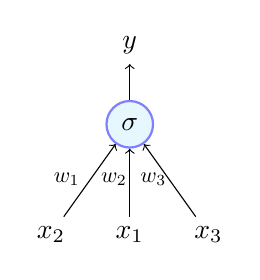
\begin{tikzpicture}
						
	\node (input0) at (10,0.6)  {$x_{1}$};
	\node (input1) at (9,0.6)  {$x_{2}$};
	\node (input2) at (11,0.6)  {$x_{3}$};
	\node [hidden_neuron] (neuron1) at (10,2)  {$\sigma$};
	
	
	\node (output0)  at (10,3) {$y$};
	
	\draw [->] (input0) -- (neuron1);
	\draw [->] (input1) -- (neuron1);
	\draw [->] (input2) -- (neuron1);
	
	\draw [->] (neuron1) -- (output0);
	
	\node (formula)[scale=.8] at (9.2,1.3) {$w_{1}$};
	\node (formula)[scale=.8] at (9.8,1.3) {$w_{2}$};
	\node (formula)[scale=.8] at (10.3,1.3) {$w_{3}$};
	
\end{tikzpicture}
				}
			\end{center}
		\end{overlayarea}
		
		
		\column{0.65\textwidth}
		\begin{overlayarea}{\textwidth}{\textheight}
			\only<1-10>{
				\begin{itemize}
					\justifying
					\onslide<2->{\item 
						We already saw how to train this network
						\vspace{-0.1in}
						\begin{align*}
							\onslide<3->{ w       & = w - \eta \nabla w \hspace{3 mm} where,}                        \\
							\onslide<4->{\nabla w & = \frac{\partial\mathscr{L}(\textbf{w})}{\partial w} }           \\
							\onslide<5->{         & = (f(\mathbf{x}) - y) * f(\mathbf{x}) * (1- f(\mathbf{x})) * x } \\
						\end{align*}
					}
					
					\only<6->{
						\onslide<6->{\item What about a wider network with more inputs:}
						\vspace{-0.1in}
						\begin{align*}
							\onslide<7->{ w_{1}               & = w_{1} - \eta \nabla w_{1}                                                         \\} 
							\onslide<8->{ w_{2}               & = w_{2} - \eta \nabla w_{2}                                                         \\}
							\onslide<9->{w_{3}                & = w_{3} - \eta \nabla w_{3}                                                         \\ } 
							\onslide<10->{where, \nabla w_{i} & = (f(\mathbf{x}) - y) * f(\mathbf{x}) * (1- f(\mathbf{x})) * \textcolor{red}{x_{i}} \\}
						\end{align*}
					}
					
				\end{itemize}
			}
			
		\end{overlayarea}
		
	\end{columns}
\end{frame}

%%%%%%%%%%%%%%%%%%%%%%%%%%%%%%%%%%%%%%%%%%%%%%%%%%%%%%%%%%%%%%%%%%%%%%%%%%%

\begin{frame}
	
	\begin{columns}
		\column{0.35\textwidth}
		\begin{overlayarea}{\textwidth}{\textheight}
			\begin{center}
				\tikzstyle{input_neuron}=[circle,draw=red!50,fill=orange!10,thick,minimum size=.2mm]
\tikzstyle{hidden_neuron}=[circle,draw=blue!50,fill=blue!10,thick,minimum size=1mm]
\tikzstyle{output_neuron}=[circle,draw=green!50,fill=green!20,thick,minimum size=1mm]
\tikzstyle{input}=[circle,draw=black!50,fill=black!20,thick,minimum size=.2mm]

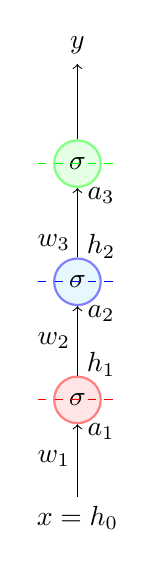
\begin{tikzpicture}

	\node [input_neuron] (neuron0) at (7,3)  {$\sigma$} ;
	\node (input0) at (7,1.5)  {$x=h_{0}$};
	
	\node [hidden_neuron] (neuron1) at (7,4.5)  {$\sigma$};
	\node [output_neuron] (neuron2) at (7,6)  {$\sigma$} ;
	
	\node (output0)  at (7,7.5) {$y$};
	
	\draw [->] (input0) -- (neuron0);
	\draw [->] (neuron0) -- (neuron1);
	\draw [->] (neuron1) -- (neuron2);
	\draw [->] (neuron2) -- (output0);
	\draw[green,dashed] (6.5,6) -- (7.5,6);
	\draw[blue,dashed] (6.5,4.5) -- (7.5,4.5);
	\draw[red,dashed] (6.5,3) -- (7.5,3);
	
	\node (formula) at (6.7,2.25) {$w_{1}$};
	\node (formula) at (6.7,3.75) {$w_{2}$};
	\node (formula) at (6.7,5.) {$w_{3}$};
	
	\node (formula) at (7.3,2.6) {$a_{1}$};
	\node (formula) at (7.3,3.45) {$h_{1}$};
	\node (formula) at (7.3,4.1) {$a_{2}$};
	\node (formula) at (7.3,4.95) {$h_{2}$};
	\node (formula) at (7.3,5.6) {$a_{3}$};
	%\node (formula) at (7.3,6.45) {$h_{3}$};
	
\end{tikzpicture}
			\end{center}
			
			\vspace{-0.4in}
			\begin{align*}
				a_{i} & =w_{i}h_{i-1}; h_{i}=\sigma{(a_{i})} \\
				a_1   & = w_1 * x = w_1 * h_0                \\
				%\frac{\partial a_{1}}{\partial w_{1}}=x
			\end{align*}
			
		\end{overlayarea}
		
		
		\column{0.65\textwidth}
		\begin{overlayarea}{\textwidth}{\textheight}
			\only<1->{
				\begin{itemize}
					\justifying
					\item What if we have a deeper network ?
					      \item<2-> We can now calculate $\nabla{w_{1}}$ using chain rule:
					      \vspace{-0.1in}
					      \begin{align*}
					      	\onslide<3->{\frac{\partial\mathscr{L}(\textbf{w})}{\partial w_{1}} & =\frac{\partial\mathscr{L}(\textbf{w})}{\partial y}.\frac{\partial y}{\partial a_{3}}.\frac{\partial a_{3}}{\partial h_{2}}.\frac{\partial h_{2}}{\partial a_{2}}.\frac{\partial a_{2}}{\partial h_{1}}.\frac{\partial h_{1}}{\partial a_{1}}.\frac{\partial a_{1}}{\partial w_{1}} \\}
					      	%\onslide<20->{\therefore \nabla{w_{1}}&=\frac{\partial\mathscr{L}(\textbf{w})}{\partial w_{1}}\\}
					      	\onslide<4->{                                                       & =\frac{\partial\mathscr{L}(\textbf{w})}{\partial y}*...............*h_0}                                                                                                                                                                                                                                                  
					      \end{align*}
					      
					      \item<5-> In general, 
					      \begin{align*}
					      	\onslide<5->{\nabla{w_{i}} & = \frac{\partial\mathscr{L}(\textbf{w})}{\partial y}*...............*\textcolor{red}{h_{i-1}} } 
					      \end{align*}
					      
					      \item<6-> Notice that $\nabla{w_{i}}$ is proportional to the corresponding input $\textcolor{red}{h_{i-1}}$  \only<7->{(we will use this fact later)}
					      
				\end{itemize}
			}
			
			
		\end{overlayarea}
		
	\end{columns}
\end{frame}


%%%%%%%%%%%%%%%%%%%%%%%%%%%%%%%%%%%%%%%%%%%%%%%%%%%%%%%%%%%%%%%%%%%%%%%%%%%%


\if 0
	\begin{frame}
		
		\begin{columns}
			\column{0.35\textwidth}
			\begin{overlayarea}{\textwidth}{\textheight}				
							
				\begin{center}
					\tikzstyle{input_neuron}=[circle,draw=red!50,fill=orange!10,thick,minimum size=.2mm]
\tikzstyle{hidden_neuron}=[circle,draw=blue!50,fill=blue!10,thick,minimum size=1mm]
\tikzstyle{output_neuron}=[circle,draw=green!50,fill=green!20,thick,minimum size=1mm]
\tikzstyle{input}=[circle,draw=black!50,fill=black!20,thick,minimum size=.2mm]
\begin{tikzpicture}

	\node [input_neuron] (neuron0) at (7,3)  {$\sigma$} ;
	\node (input0) at (7,1.5)  {$x=h_{0}$};
	
	\node [hidden_neuron] (neuron1) at (7,4.5)  {$\sigma$};
	\node [output_neuron] (neuron2) at (7,6)  {$\sigma$} ;
	
	\node (output0)  at (7,7.5) {$y$};
	
	\draw [->] (input0) -- (neuron0);
	\draw [->] (neuron0) -- (neuron1);
	\draw [->] (neuron1) -- (neuron2);
	\draw [->] (neuron2) -- (output0);
	\only<16->{\draw[green,dashed] (6.5,6) -- (7.5,6);}
	\only<11->{\draw[blue,dashed] (6.5,4.5) -- (7.5,4.5);}
	\only<6->{\draw[red,dashed] (6.5,3) -- (7.5,3);}
	
	\node (formula) at (6.7,2.25) {$w_{1}$};
	\node (formula) at (6.7,3.75) {$w_{2}$};
	\node (formula) at (6.7,5.) {$w_{3}$};
	
	\only<7->{\node (formula) at (7.3,2.6) {$a_{1}$};}
	\only<9->{\node (formula) at (7.3,3.45) {$h_{1}$};}
	\only<12->{\node (formula) at (7.3,4.1) {$a_{2}$};}
	\only<14->{\node (formula) at (7.3,4.95) {$h_{2}$};}
	\only<16->{\node (formula) at (7.3,5.6) {$a_{3}$};}
	\only<16->{\node (formula) at (7.3,6.45) {$h_{3}$};}
	
\end{tikzpicture}
				\end{center}
				
				\vspace{-0.4in}
				\begin{align*}
					\only<8-12>{a_{1}  & =w_{1}h_{0};} \only<10-12>{h_{1}=\sigma{(a_{1})} \\}
					\only<13-16>{a_{2} & =w_{2}h_{1};} \only<15-16>{h_{2}=\sigma{(a_{2})} \\}
					\only<17->{a_{i}   & =w_{i}h_{i-1};} \only<17->{h_{i}=\sigma{(a_{i})} \\}
					\only<20->{a_1     & = w_1 * x = w_1 * h_0                            \\}
					%\frac{\partial a_{1}}{\partial w_{1}}=x
				\end{align*}
				
			\end{overlayarea}
			
			
			\column{0.65\textwidth}
			\begin{overlayarea}{\textwidth}{\textheight}
				\only<1-17>{
					\begin{itemize}
						\justifying
						\item What if we have a deeper network:
						      \begin{align*}
						      	\onslide<1->{ w_{1} & = w_{1} - \eta \nabla w_{1}} \\
						      	\onslide<2->{ w_{2} & = w_{2} - \eta \nabla w_{2}} \\
						      	\onslide<3->{w_{3}  & = w_{3} - \eta \nabla w_{3}} \\ 
						      \end{align*}
						      
						      \onslide<4->{\item  But what does $\nabla{w_{1}}$ look like now?}
						      \onslide<5->{\item  Let's define some notations before answering this!}
					\end{itemize}
				}
				
				\only<18->{
					\begin{itemize}
						\justifying
						\only<18->{
							\item<18-> We can now calculate $\nabla{w_{1}}$ using chain rule:
							\vspace{-0.1in}
							\begin{align*}
								\onslide<19->{\frac{\partial\mathscr{L}(\textbf{w})}{\partial w_{1}} & =\frac{\partial\mathscr{L}(\textbf{w})}{\partial y}.\frac{\partial y}{\partial h_{3}}.\frac{\partial h_{3}}{\partial a_{3}}.\frac{\partial a_{3}}{\partial h_{2}}.\frac{\partial h_{2}}{\partial a_{2}}.\frac{\partial a_{2}}{\partial h_{1}}.\frac{\partial h_{1}}{\partial a_{1}}.\frac{\partial a_{1}}{\partial w_{1}} \\}
								%\onslide<20->{\therefore \nabla{w_{1}}&=\frac{\partial\mathscr{L}(\textbf{w})}{\partial w_{1}}\\}
								\onslide<20->{                                                       & =\frac{\partial\mathscr{L}(\textbf{w})}{\partial y}*...............*h_0}                                                                                                                                                                                                                                                  
							\end{align*}
							
							\item<21-> In general, 
							\begin{align*}
								\onslide<21->{\nabla{w_{i}} & = \frac{\partial\mathscr{L}(\textbf{w})}{\partial y}*...............*\textcolor{red}{h_{i-1}} } 
							\end{align*}
							
							\item<22-> Notice that $\nabla{w_{i}}$ is proportional to the corresponding input $\textcolor{red}{h_{i-1}}$  \only<23->{(we will use this fact later)}
						}
					\end{itemize}
				}
				
				
			\end{overlayarea}
			
		\end{columns}
	\end{frame}
\fi 

%%%%%%%%%%%%%%%%%%%%%%%%%%%%%%%%%%%%%%%%%%%%%%%%%%%%%%%%%%%%%%%%%%%%%%%%%%%

\begin{frame}
	
	\begin{columns}
		\column{0.35\textwidth}
		\begin{overlayarea}{\textwidth}{\textheight}	
			\tikzstyle{input_neuron}=[circle,draw=red!50,fill=orange!10,thick,minimum size=.2mm]
\tikzstyle{hidden_neuron}=[circle,draw=blue!50,fill=blue!10,thick,minimum size=1mm]
\tikzstyle{output_neuron}=[circle,draw=green!50,fill=green!20,thick,minimum size=1mm]
\tikzstyle{input}=[circle,draw=black!50,fill=black!20,thick,minimum size=.2mm]
\begin{tikzpicture}

	\node [output_neuron] (out0) at (5,7)  {$\sigma$} ;
	
	\node [input_neuron] (in0) at (4,4)  {$\sigma$} ;
	\node (input0) at (4,3)  {$x_1$};
	\node [input_neuron] (in1) at (5,4)  {$\sigma$};
	\node [input_neuron] (in2) at (6,4)  {$\sigma$} ;
	\node (input1)  at (5,3) {$x_2$};
	\node (input2)  at (6,3) {$x_3$};
	
	\node [hidden_neuron] (hi0) at (4,5)  {$\sigma$} ;
	\node [hidden_neuron] (hi1) at (5,5)  {$\sigma$};
	\node [hidden_neuron] (hi2) at (6,5)  {$\sigma$} ;
	
	%\node [hidden_neuron] (hi3) at (4,6)  {$\sigma$} ;
	\node [hidden_neuron] (hi4) at (5,6)  {$\sigma$};
	%\node [hidden_neuron] (hi5) at (6,6)  {$\sigma$} ;
	
	\node (output0) (output0) at (5,8)  {$y$} ;
	
	
	\draw [->] (input0) -- (in0);
	\draw [->](input1) -- (in1);
	\draw [->] (input2) -- (in2);
	\draw [->] (in0) -- (hi0);
	\draw [->] (in0) -- (hi1);
	\draw [->] (in0) -- (hi2);
	\draw [->](in1) -- (hi0);
	\draw [->](in1) -- (hi1);
	\draw [->](in1) -- (hi2);
	\draw [->] (in2) -- (hi0);
	\draw [->] (in2) -- (hi1);
	\draw [->] (in2) -- (hi2);
	
	%\draw [->](hi0) -- (hi3);
	\draw [->](hi0) -- (hi4);
	%\draw [->](hi0) -- (hi5);
	%\draw [->](hi1) -- (hi3);
	\draw [->](hi1) -- (hi4);
	%\draw [->] (hi1) -- (hi5);
	%\draw [->] (hi2) -- (hi3);
	\draw [->] (hi2) -- (hi4);
	%\draw [->] (hi2) -- (hi5);
	
	\draw [->] (hi4) -- (out0);
	%\draw [->] (hi3) -- (out0);
	%\draw [->] (hi5) -- (out0);
	
	
	\draw [->] (out0) -- (output0);
	\only<4->{\draw [->][line width=0.75mm,red] (output0) -- (out0);}
	
	\node (formula) at (3.7,3.5) {$w_{1}$};
	\node (formula) at (4.7,3.5) {$w_{2}$};
	\node (formula) at (5.7,3.5) {$w_{3}$};
	
	\if 0
		\only<3->{\draw[red] [->](hi0) -- (hi3);
			\draw[red] [->](input1) -- (in1);
			\draw[red] [->](in1) -- (hi0);
			\draw[red] [->](hi3) -- (out0);
		}
	\fi
	
	\only<5->{\draw[line width=0.75mm,red] [->](hi4) -- (hi0);
		\draw[line width=0.75mm,red] [->](in1) -- (input1);
		\draw[line width=0.75mm,red] [->](hi0) -- (in1);
		\draw[line width=0.75mm,red] [->](out0) -- (hi4);
	}
	
	\if 0
		\only<5->{\draw[red] [->](hi0) -- (hi5);
			\draw[red] [->](input1) -- (in1);
			\draw[red] [->](in1) -- (hi0);
			\draw[red] [->](hi5) -- (out0);
		}
		
		
		\only<6->{\draw[red] [->](hi1) -- (hi3);
			\draw[red] [->](input1) -- (in1);
			\draw[red] [->](in1) -- (hi1);
			\draw[red] [->](hi3) -- (out0);
		}
	\fi
	
	\only<4->{\draw[line width=0.75mm,red] [->](hi4) -- (hi1);
		\draw[line width=0.75mm,red] [->](in1) -- (input1);
		\draw[line width=0.75mm,red] [->](hi1) -- (in1);
		\draw[line width=0.75mm,red] [->](out0) -- (hi4);
	}
	
	\if 0
		\only<8->{\draw[red] [->](hi1) -- (hi5);
			\draw[red] [->](input1) -- (in1);
			\draw[red] [->](in1) -- (hi1);
			\draw[red] [->](hi5) -- (out0);
		}
		\only<9->{\draw[red] [->](hi2) -- (hi3);
			\draw[red] [->](input1) -- (in1);
			\draw[red] [->](in1) -- (hi2);
			\draw[red] [->](hi3) -- (out0);
		}
	\fi
	
	\only<6->{\draw[line width=0.75mm,red] [->](hi4) -- (hi2);
		\draw[line width=0.75mm,red] [->](in1) -- (input1);
		\draw[line width=0.75mm,red] [->](hi2) -- (in1);
		\draw[line width=0.75mm,red] [->](out0) -- (hi4);
	}
	\if 0
		\only<11->{\draw[red] [->](hi2) -- (hi5);
			\draw[red] [->](input1) -- (in1);
			\draw[red] [->](in1) -- (hi2);
			\draw[red] [->](hi5) -- (out0);
		}
	\fi
	%\draw (6.5,7) -- (7.5,7);
	%\draw (6.5,6) -- (7.5,6);
	%\draw (6.5,5) -- (7.5,5);
\end{tikzpicture}	
		\end{overlayarea}
		
		\column{0.65\textwidth}
		\begin{overlayarea}{\textwidth}{\textheight}
			
			\begin{itemize}
				\justifying
				\item<1-> What happens if we have a network which is deep and wide?		
				\item<2-> How do you calculate $\nabla{w_{2}}=?$
				\item<3-> It will be given by chain rule applied across multiple paths \only<7->{(We saw this in detail when we studied \textbf{back propagation})}
			\end{itemize}
			
		\end{overlayarea}
		
	\end{columns}
\end{frame}

%%%%%%%%%%%%%%%%%%%%%%%%%%%%%%%%%%%%%%%%%%%%%%%%%%%%%%%%%%%%%%%%%%%%%%%%

\begin{frame}
	\vspace{.35in}
	\begin{overlayarea}{\textwidth}{\textheight}
		\begin{block}{Things to remember}
			\begin{itemize}
				\justifying
				\onslide<1->{\item Training Neural Networks is a \textit{\textbf{Game of Gradients}} (played using any of the existing gradient based approaches that we discussed)}
				\onslide<2->{\item The gradient tells us the responsibility of a parameter towards the loss}
				\onslide<3->{\item The gradient w.r.t. a parameter is proportional to the input to the parameters (recall the ``$.....*x$" term or the ``$....*h_{i}$" term in the formula for $\nabla{w_i}$) }
			\end{itemize}
		\end{block}
	\end{overlayarea}
\end{frame}

%%%%%%%%%%%%%%%%%%%%%%%%%%%%%%%%%%%%%%%%%%%%%%%%%%%%%%%%%%%%%%%%%%%5

\begin{frame}
	\begin{columns}
		
		\column{0.5\textwidth}
		\begin{overlayarea}{\textwidth}{\textheight}
			\vspace{1cm}
			\begin{center}		
				\tikzstyle{input_neuron}=[circle,draw=red!50,fill=orange!10,thick,minimum size=.2mm]
\tikzstyle{hidden_neuron}=[circle,draw=blue!50,fill=blue!10,thick,minimum size=1mm]
\tikzstyle{output_neuron}=[circle,draw=green!50,fill=green!20,thick,minimum size=1mm]
\tikzstyle{input}=[circle,draw=black!50,fill=black!20,thick,minimum size=.2mm]

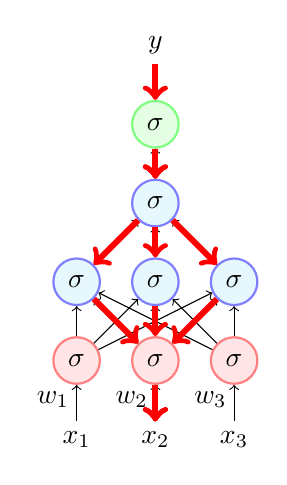
\begin{tikzpicture}

	\node [output_neuron] (out0) at (5,7)  {$\sigma$} ;
	
	\node [input_neuron] (in0) at (4,4)  {$\sigma$} ;
	\node (input0) at (4,3)  {$x_1$};
	\node [input_neuron] (in1) at (5,4)  {$\sigma$};
	\node [input_neuron] (in2) at (6,4)  {$\sigma$} ;
	\node (input1)  at (5,3) {$x_2$};
	\node (input2)  at (6,3) {$x_3$};
	
	\node [hidden_neuron] (hi0) at (4,5)  {$\sigma$} ;
	\node [hidden_neuron] (hi1) at (5,5)  {$\sigma$};
	\node [hidden_neuron] (hi2) at (6,5)  {$\sigma$} ;
	
	%\node [hidden_neuron] (hi3) at (4,6)  {$\sigma$} ;
	\node [hidden_neuron] (hi4) at (5,6)  {$\sigma$};
	%\node [hidden_neuron] (hi5) at (6,6)  {$\sigma$} ;
	
	\node (output0) (output0) at (5,8)  {$y$} ;
	
	
	\draw [->] (input0) -- (in0);
	\draw [->](input1) -- (in1);
	\draw [->] (input2) -- (in2);
	\draw [->] (in0) -- (hi0);
	\draw [->] (in0) -- (hi1);
	\draw [->] (in0) -- (hi2);
	\draw [->](in1) -- (hi0);
	\draw [->](in1) -- (hi1);
	\draw [->](in1) -- (hi2);
	\draw [->] (in2) -- (hi0);
	\draw [->] (in2) -- (hi1);
	\draw [->] (in2) -- (hi2);
	
	%\draw [->](hi0) -- (hi3);
	\draw [->](hi0) -- (hi4);
	%\draw [->](hi0) -- (hi5);
	%\draw [->](hi1) -- (hi3);
	\draw [->](hi1) -- (hi4);
	%\draw [->] (hi1) -- (hi5);
	%\draw [->] (hi2) -- (hi3);
	\draw [->] (hi2) -- (hi4);
	%\draw [->] (hi2) -- (hi5);
	
	\draw [->] (hi4) -- (out0);
	%\draw [->] (hi3) -- (out0);
	%\draw [->] (hi5) -- (out0);
	
	
	%\draw [->] (out0) -- (output0);
	\draw [->][line width=0.75mm,red] (output0) -- (out0);
	
	\node (formula) at (3.7,3.5) {$w_{1}$};
	\node (formula) at (4.7,3.5) {$w_{2}$};
	\node (formula) at (5.7,3.5) {$w_{3}$};
	
	
	\draw[line width=0.75mm,red] [->](hi4) -- (hi0);
	\draw[line width=0.75mm,red] [->](in1) -- (input1);
	\draw[line width=0.75mm,red] [->](hi0) -- (in1);
	\draw[line width=0.75mm,red] [->](out0) -- (hi4);
	
	
	\draw[line width=0.75mm,red] [->](hi4) -- (hi1);
	\draw[line width=0.75mm,red] [->](in1) -- (input1);
	\draw[line width=0.75mm,red] [->](hi1) -- (in1);
	\draw[line width=0.75mm,red] [->](out0) -- (hi4);
	
	\draw[line width=0.75mm,red] [->](hi4) -- (hi2);
	\draw[line width=0.75mm,red] [->](in1) -- (input1);
	\draw[line width=0.75mm,red] [->](hi2) -- (in1);
	\draw[line width=0.75mm,red] [->](out0) -- (hi4);
	%\draw (6.5,7) -- (7.5,7);
	%\draw (6.5,6) -- (7.5,6);
	%\draw (6.5,5) -- (7.5,5);
	
\end{tikzpicture}
			\end{center}
		\end{overlayarea}
		
		\column{0.5\textwidth}
		\begin{overlayarea}{\textwidth}{\textheight}
			\vspace{0.1cm}
			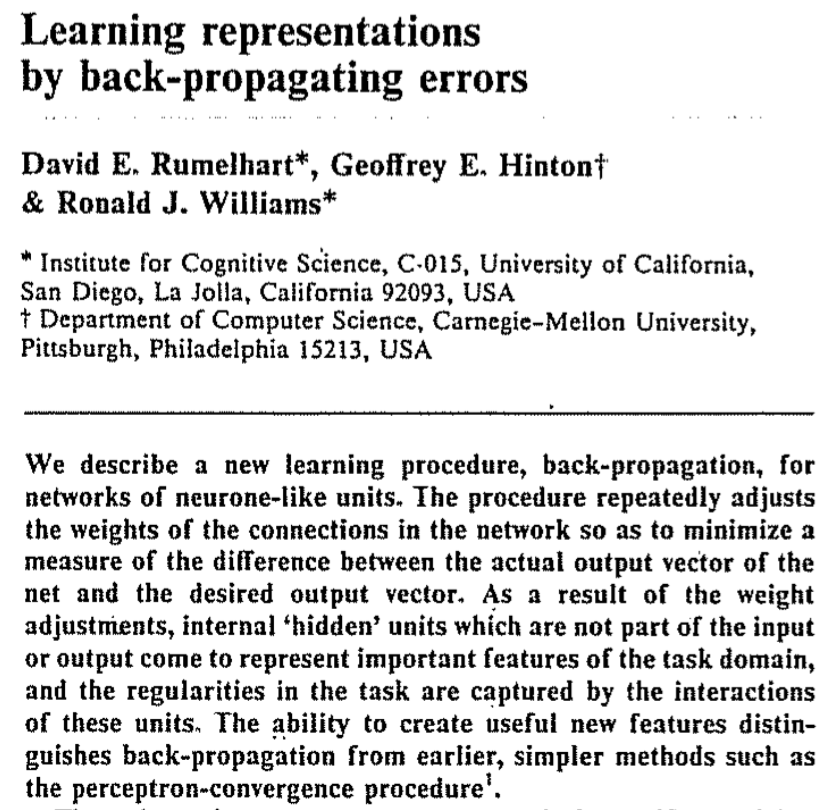
\includegraphics[width=4cm,height=3cm]{images/BackProp_paper.png}
			\begin{itemize}[<+(1)->]
				\justifying
				\item Backpropagation was made popular by Rumelhart et.al in 1986
				\item However when used for really deep networks it was not very successful
				\item In fact, till 2006 it was very hard to train very deep networks
				      %\item Let us see one intuitive reason for why this was the case
				\item Typically, even after a large number of epochs the training did not converge
			\end{itemize}
			
		\end{overlayarea}
	\end{columns}
	
\end{frame}

\if 0
	\begin{frame}
		\begin{columns}
			\column{0.35\textwidth}
			\begin{center}
				\tikzstyle{input_neuron}=[circle,draw=red!50,fill=red!10,thick,minimum size=.2mm]
\tikzstyle{hidden_neuron}=[circle,draw=blue!50,fill=cyan!10,thick,minimum size=1mm]
\tikzstyle{output_neuron}=[circle,draw=green!50,fill=green!10,thick,minimum size=1mm]
\tikzstyle{input}=[circle,draw=black!50,fill=black!20,thick,minimum size=1.5mm]

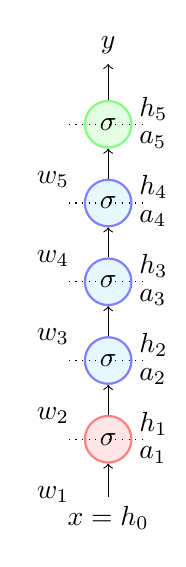
\begin{tikzpicture}

	\node [input_neuron] (neuron0) at (7,5)  {$\sigma$} ;
	\node (input0) at (7,4)  {$x=h_0$};
	
	\node [hidden_neuron] (neuron1) at (7,6)  {$\sigma$};
	\node [hidden_neuron] (neuron2) at (7,7)  {$\sigma$};
	\node [hidden_neuron] (neuron3) at (7,8)  {$\sigma$};
	\node [output_neuron] (neuron4) at (7,9)  {$\sigma$} ;
	
	\node (output0)  at (7,10) {$y$};
	
	\draw [->] (input0) -- (neuron0);
	\draw [->] (neuron0) -- (neuron1);
	\draw [->] (neuron1) -- (neuron2);
	\draw [->] (neuron2) -- (neuron3);
	\draw [->] (neuron3) -- (neuron4);
	\draw [->] (neuron4) -- (output0);
	\draw [dotted] (6.5,5) -- (7.5,5);
	\draw [dotted] (6.5,6) -- (7.5,6);
	\draw [dotted] (6.5,7) -- (7.5,7);
	\draw [dotted] (6.5,8) -- (7.5,8);
	\draw [dotted] (6.5,9) -- (7.5,9);
	\node[text width=0.01cm] at (6.1,4.3) {$w_1$};
	\node[text width=0.01cm] at (6.1,5.3) {$w_2$};
	\node[text width=0.01cm] at (6.1,6.3) {$w_3$};
	\node[text width=0.01cm] at (6.1,7.3) {$w_4$};
	\node[text width=0.01cm] at (6.1,8.3) {$w_5$};
	
	
	\node[text width=0.01cm] at (7.4,4.8) {$a_1$};
	\node[text width=0.01cm] at (7.4,5.2) {$h_1$};
	\node[text width=0.01cm] at (7.4,5.8) {$a_2$};
	\node[text width=0.01cm] at (7.4,6.2) {$h_2$};
	\node[text width=0.01cm] at (7.4,6.8) {$a_3$};
	\node[text width=0.01cm] at (7.4,7.2) {$h_3$};
	\node[text width=0.01cm] at (7.4,7.8) {$a_4$};
	\node[text width=0.01cm] at (7.4,8.2) {$h_4$};
	\node[text width=0.01cm] at (7.4,8.8) {$a_5$};
	\node[text width=0.01cm] at (7.4,9.2) {$h_5$};
	
\end{tikzpicture}
			\end{center}
			
			\column{0.65\textwidth}
			\begin{overlayarea}{\textwidth}{\textheight}
				\vspace{0.1cm}
				
				%$\frac{\partial h(w)}{\partial w_1} = \frac{\partial h(w)}{\partial y}\frac{\partial y}{\partial h_5} \hspace{0.3 cm} {\Sigma_{i=1}^{5} }\frac{\partial h_i}{\partial a_i}  \frac{\partial a_i }{\partial h_{i-1}}$
				
				\begin{align*}
					\frac{\partial \mathscr{L}(\textbf{w})} {\partial w_1} = \frac{\partial h(w)}{\partial y} \frac{\partial y}{\partial h_5} {\prod_{i=1}^{5} }\frac{\partial h_i}{\partial a_i}  \frac{\partial a_i }{\partial h_{i-1}} 
				\end{align*}
				
				
				
				\begin{itemize}[<+(1)->]
					\justifying
					\item If each term in the product is $\textless$ 1 then the multiplicative effect will cause 
					      $\frac{\partial \mathscr{L}(\textbf{w})} {\partial w_1}$   $\rightarrow$ 0   
					\item In other words, the gradient $\nabla w $ will vanish
					      \begin{align*}
					      	w & = w-\eta\nabla w                    \\ 
					      	  & =w \quad (if \nabla w\rightarrow 0) 
					      \end{align*}
					\item Hence $w$ will not change much from its initial random value and the network will not train
				\end{itemize}
				
				
			\end{overlayarea}
		\end{columns}
		
	\end{frame}
\fi